  \textbf{Results on GPU and CPU load balance}: Fig.~\ref{figs:cpu-gpu-balance} 
  shows two time steps of the timeline of running DHFR using 4 CPU cores and 1 GPU. 
  In the first time step, all work is offload to GPU, which is the original design.
  The time cost for this step is $848 ms$. After applying the new balance scheme
  we discussed in section~\ref{sec:balance}, the time line is shown in the second step.
  We can see that all 4 CPU cores and the GPU is kept busy all the time. The time step 
  is $178 ms$, which is 4.8x speedup.
On Blue Waters, we achieved speedup of 1.3x due to the fast GPU.

\begin{figure}[h]
\centering
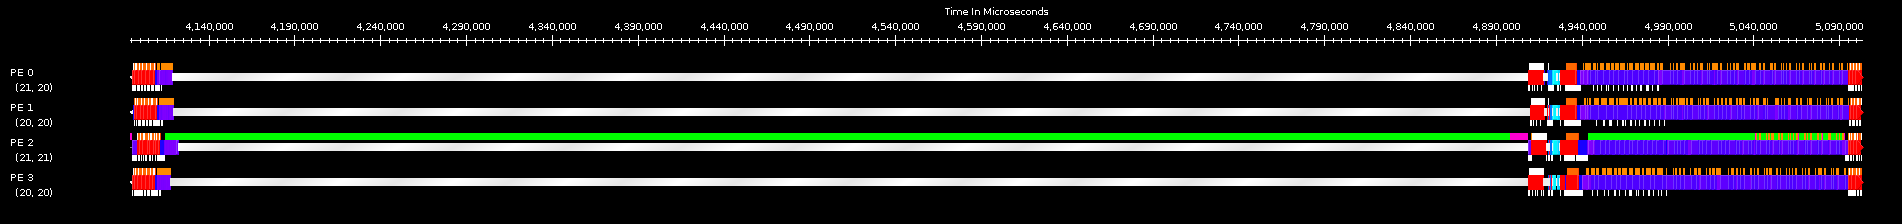
\includegraphics[width=6.5in]{figs/gpu-cpu-balance-timeline.png}
\caption{Timeline of running DHFR before and after load balance}
\label{figs:cpu-gpu-balance}
\end{figure}

\textbf{GPU kernel optimization results}. So far, we did not see performance improvement using 
our optimization. Main reason is that we used more shared memory than the original version 
so that the occupancy is lower than before. We are still working on it.
